\chapter{Planificación del trabajo y presupuesto}
\section{Planificación del trabajo}
\subsection{Definición de tareas}
La elaboración del presente proyecto se ha dividido en tres fases, que se enumeran a continuaón:
\begin{itemize}
  \item \underline{FASE 1: Planificación}  \hfill  \\
  En todo proyecto antes de empezar a trabajar es necesario un estudio previo de los requisitos necesarios y de las posibles tecnologías para desarrollar el trabajo.
  \begin{itemize}
    \item \textit{Planteamiento del trabajo: }La primera tarea consistió en estudiar cuales eran los objetivos necesarios para la realización de este proyecto, su finalidad y una previa organización del mismo.
    \item \textit{Definición de requisitos: }Una vez examinados los objetivos indispensables, se realizó un listado de los requisitos tanto técnicos como materiales necesarios para llevar a cabo este proyecto.
    \item \textit{Estudio de sistemas de desarrollo: } El siguiente paso fue el análisis de las diferentes
alternativas para desarrollar este trabajo fin de grado, definiendo que lenguaje de programación utilizar, las tecnologías adecuadas, y la elección de la base de datos.
    \item \textit{Estudio de las tecnologías web: } Por último, se estudiaron las diferentes tecnologías web disponibles para desarrollar el portal web y las opciones que más convenían para este proyecto.
  \end{itemize}
  \item \underline{FASE 2: Desarrollo} \hfill \\
  
  2.1 BACKEND    
  \begin{itemize}
    \item \textit{Creación de las bases de datos:} Definido el proyecto, se empezó creando las bases de datos necesarias, una en MongoDB y otra en MySQL. Los requisitos de las bases de datos creadas se fueron incrementando en función de las necesidades de los programas que acceden a ellas.
    \item \textit{Creación script API de Facebook: } Después de crear un primer esquema de las bases de datos, el siguiente paso fue la realización del script que accedía a la API de Facebook. Hubo que analizar las diferentes posibilidades de acceder a la API de Facebook, los parámetros necesarios y la configuración adecuada.
    \item \textit{Creación del \textit{crawler} de Facebook: } Realizadas las primeras pruebas del script de la API de Facebook y teniendo los primeros datos para poder seguir avanzando con el proyecto, se procedió a desarrollar el \textit{crawler}, tarea que requería mayor tiempo de dedicación.
    \item \textit{Distribución del \textit{crawler} en distintas máquinas virtuales: }Desarrollado el \textit{crawler} casi por completo, se decidió montar una estructura para dividir el \textit{crawler} automáticamente en varias máquinas virtuales. Para esta parte se desarrolló un sistema de colas de mensajes con RabbitMQ que supuso también mucho tiempo de pruebas pero ayudó a definir mejor los requisitos del \textit{crawler}.
    \end{itemize}
    
    2.2 FRONTEND
    \begin{itemize}
    \item \textit{Implementación del diseño de la aplicación web: } En cuanto al \textit{frontend}, lo primero que se realizó fue una primera plantilla sencilla con un formulario que fuera capaz de introducir los datos indicados por un usuario en una base de datos. Una vez conseguido esto, se decidió el diseño de la web y se mejoraron
aspectos de estilo.
    \item \textit{Implementación del registro de usuarios: }Definidas las funcionalidades básicas de la aplicación web, se creó un sistema de registro/autenticación, para que sólo los usuarios registrados pudieran tener acceso a la aplicación.
    \item \textit{Implementación de las funcionalidades de la aplicación: } Una vez desarrolladas todas las partes necesarias para la creación de este proyecto, sólo faltaba unir los script creados en el \textit{backend} con la aplicación para que automáticamente parseará y obtuviera los datos de Facebook, los procesara y se los mostrara al usuario en la interfaz gráfica.
  \end{itemize}
  \item \underline{FASE 3: Evaluación y documentación} \hfill  \\
  El último bloque para finalizar el desarrollo de este trabajo fin de grado consistía en realizar pruebas de la aplicación y la redacción de la presente memoria, así como la preparación de la presentación del mismo.
    \begin{itemize}
    \item \textit{Pruebas aplicación:} Finalizado el sistema completo, se realizaron pruebas para comprobar el correcto funcionamiento y se llevaron a cabo un par de casos prácticos para explicar su funcionamiento en el presente documento.  
    \item \textit{Redacción de la memoria: } Redacción del presente documento.
    \item \textit{Preparación de la presentación.}
  \end{itemize}  
\end{itemize}

\subsection{Planificación: Diagrama de Gantt}
Una vez establecidas las tareas principales que definen el proyecto, se enmarcan dichas tareas en un intervalo temporal para establecer el tiempo estimado en la realización del mismo. Este periodo de tiempo se estima teniendo en cuenta el plazo máximo de entrega del proyecto, el 27 de Septiembre, y la disponibilidad del autor para la realización del trabajo. En este caso concreto, se ha requerido más tiempo ya que no se realizó a jornada completa.

En el diagrama de Gantt (\ref{tab:gantt}) se representan cada una de las fases definidas con el periodo de tiempo estimado. Se ha considerado el tiempo máximo disponible, 9 meses.
\begin{table}[H]
	\centering
	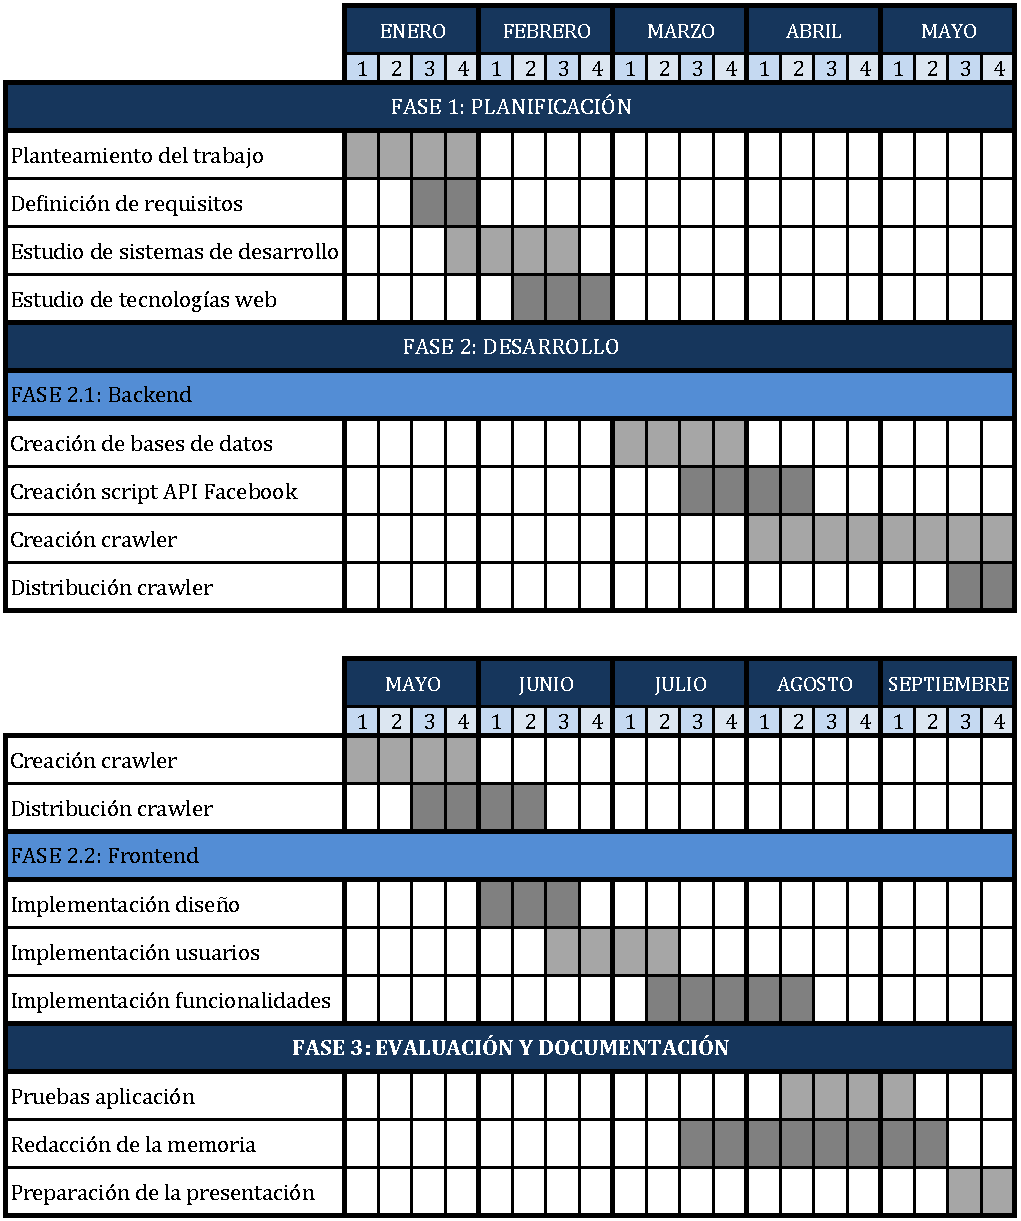
\includegraphics[width=6in]{PDF/DiagramadeGantt.pdf}
	\caption{Planificación del proyecto. Diagrama de Gantt}
	\label{tab:gantt}
\end{table}

\section{Presupuesto}
En el siguiente apartado se procede al calculo del presupuesto del proyecto realizado, detallando dos tipos de costes: costes materiales y costes de personal.
\subsection{Costes materiales}
En cuanto a costes materiales se han tenido en cuenta las siguientes variables:
\begin{itemize}
\item Portátil: Ordenador portátil de uso personal, marca Apple y modelo MacBook Air.
\item Software: El software utilizado para la realización del proyecto es de código abierto. Sólo se tiene en cuenta la utilización del paquete Microsoft Office para la realización de la documentación del proyecto. 
\item Servidor: Donde alojar OpenStack.
\item Material de oficina: Varios.
\item Alquiler de oficina: Estudio estimado de unos 20 metros cuadrados en Madrid. 
\item Gastos de luz y de internet.
\end{itemize}
\subsection{Costes de personal}
En cuanto a los costes de personal, se ha tenido en cuenta las horas dedicadas por parte del tutor, considerando el precio de la hora como Ingeniero Senior, y las horas dedicadas por parte de la autora del presente proyecto, contando las horas como Ingeniero Junior. 

Para estimar el precio de estas horas, según el Colegio de Ingenieros Técnicos de Telecomunicación (COITT) \cite{6}: \textit{"los honorarios son libres y responden al libre acuerdo entre el profesional y su cliente"}. 
\subsection{Costes totales}
En la siguiente tabla (\ref{tab:pres}) se calcula el presupuesto total del proyecto, teniendo en cuenta los costes comentados anteriormente. 
\begin{table}[H]
	\centering
	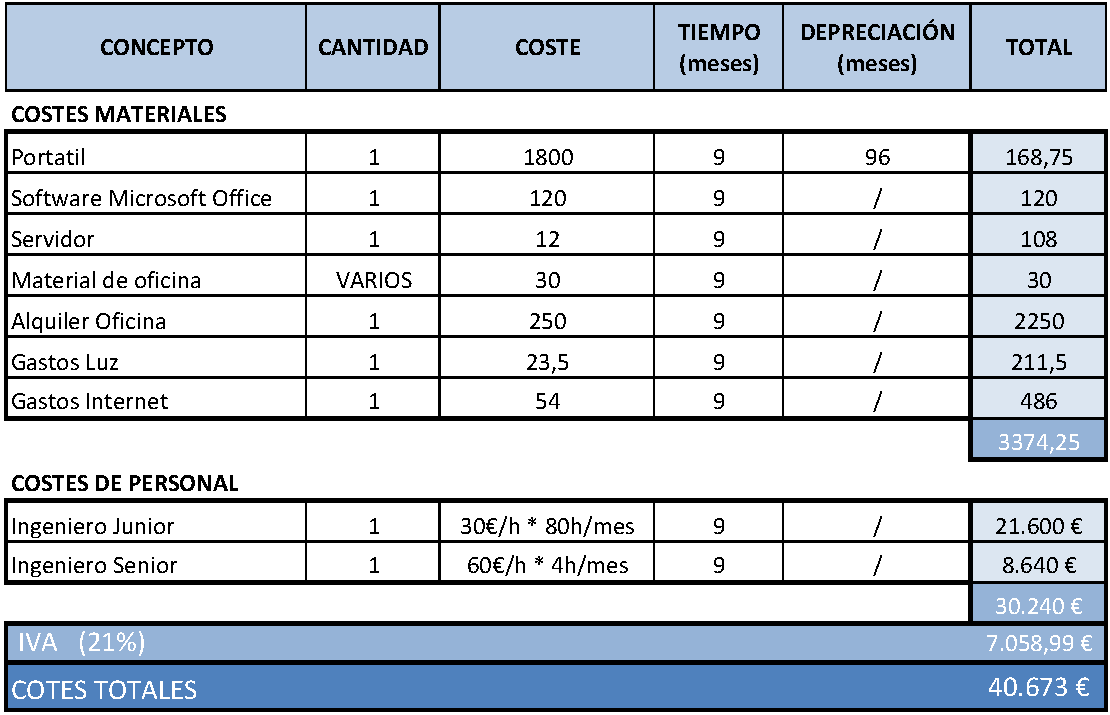
\includegraphics[width=5in]{PDF/Presupuesto.pdf}
	\caption{Presupuesto del proyecto}
	\label{tab:pres}
\end{table}